%----------------------------------------------------------------------------------------
%	PACKAGES AND OTHER DOCUMENT CONFIGURATIONS
%----------------------------------------------------------------------------------------

\documentclass[12pt]{article}

\usepackage{polski}
\usepackage[polish]{babel}
\usepackage[utf8]{inputenc}
\usepackage{datetime} 
\usepackage{graphicx} 
\usepackage{tikz}
\usepackage{amsmath} 
\usepackage{epstopdf}
\usepackage{multirow}
\usepackage{tabularx}
%\usepackage[colorlinks=true]{hyperref}
%\usepackage[all]{hypcap}
%\usepackage{showframe} 
\usepackage{geometry}
 \geometry{
 	a4paper, 
 	left	=20mm,
 	right	=20mm,
 	top		=20mm,
 	bottom	=20mm,
 }
 
%----------------------------------------------------------------------------------------
 
%----------------------------------------------------------------------------------------
% DATES
%----------------------------------------------------------------------------------------

\renewcommand{\dateseparator}{.}
\newdate{exercise_date}{01}{12}{2014}

%----------------------------------------------------------------------------------------

%----------------------------------------------------------------------------------------
% TIKZ PACKAGES
%----------------------------------------------------------------------------------------

\usetikzlibrary{arrows}

%----------------------------------------------------------------------------------------

\begin{document}
 
\begin{titlepage}

\newcommand{\HRule}{\rule{\linewidth}{0.5mm}}
% Defines a new command for the horizontal lines, change thickness here

\center
% Center everything on the page
 
%----------------------------------------------------------------------------------------
%	LOGO SECTION
%----------------------------------------------------------------------------------------

\includegraphics[width=6cm]{../res/img/logo.png}\\[1cm]
% Include a department/university logo - this will require the graphicx package
 
%----------------------------------------------------------------------------------------
 
%----------------------------------------------------------------------------------------
%	HEADING SECTIONS
%----------------------------------------------------------------------------------------

\textsc{\LARGE Akademia Górniczo-Hutnicza \\[0.2cm]
im. Stanisława Staszica w Krakowie}\\[1.5cm]
% Name of your university/college

\textrm{\Large Wydział Elektrotechniki Automatyki Informatyki i Inżynierii
Biomedycznej}\\[1cm]

\textsc{\Large Laboratorium Aparatury Automatyzacji}\\[0.5cm]
% Major heading such as course name

%----------------------------------------------------------------------------------------
%	TITLE SECTION
%----------------------------------------------------------------------------------------

\HRule \\[0.4cm]
{ \huge \bfseries Prosty regulator mikroprocesorowy 
}\\%[0.4cm]
% Title of your document
\HRule \\[1.5cm]

%----------------------------------------------------------------------------------------
%	REPORT TABLE
%----------------------------------------------------------------------------------------

\begin{table}[h]
\centering
\begin{tabularx}{\linewidth}{|c|l|X|}
\hline
% \multicolumn{3}{|c|}{
% \begin{tabular}{cc}
% \begin{tabular}{c}
% \includegraphics[height=2.2cm]{../res/img/logo.jpg}\\
% \end{tabular}
% &
% \begin{tabular}{c}
% \Large{Akademia Górniczo-Hutnicza im. Stanisława Staszica}\\[5pt]
% \large{\textsc{Katedra Automatyki}}\\[5pt]
% \textsc{Laboratorium Aparatury Automatyzacji}
% \end{tabular}
% \end{tabular}
% }\\
% \hline
% \multicolumn{3}{|c|}{}\\[-5pt]
% \multicolumn{3}{|c|}{\textbf{\huge{Ćwiczenie 6}}}\\[10pt]
% \multicolumn{3}{|c|}{\Large{Bezpośrednie sterowanie cyfrowe}}\\[8pt]
% \hline
\multicolumn{2}{|c|}{Wydział EAIiIB, kierunek AiR, rok II}
& Grupa 6, wtorek 11:00-12:30\\
\hline
Lp. & Imię i nazwisko & Zaliczenie\\
\hline
1 & \textbf{Konrad Adasiewicz} & \\
\hline
2 & \textbf{Michał Maciejewski} & \\
\hline
3 & \textbf{Bartosz Szmit} & \\
\hline
\multicolumn{2}{|c|}{Data wykonania ćwiczenia:
\ddmmyyyydate\displaydate{exercise_date}r.} & Data oddania sprawozdania:
\ddmmyyyydate\displaydate{create_date}r.
\\
\hline
\end{tabularx}
\end{table}

%----------------------------------------------------------------------------------------

\vfill % Fill the rest of the page with whitespace

\end{titlepage} 

% Program ćwiczenia

\begin{section}{Program ćwiczenia}
	\begin{enumerate}
	  	\item Budowa i konfigurowanie toru do pomiaru przyśpieszenia na bazie
	  	tensometrycznego czujnika przyśpieszenia typu BWH i wzmacniacza
	  	tensometrycznego MVD2555, skalowanie czujnika w oparciu o przyspieszenie
	  	ziemskie.
		\item Budowa i konfigurowanie toru pomiarowego do pomiaru przyśpieszenia na
		bazie zintegrowanych, pojemnościowych czujników przyśpieszenia typu ADXL320EB
		w układzie trójosiowym i karty pomiarowej, skalowanie czujnika w osiach x, y,
		z w oparciu o przyśpieszenie ziemskie.
		\item Opracowanie systemu pomiarowego w środowisku DASYLab, rejestracja
		sygnałów drgań silnika oraz wyznaczenie i analiza widma sygnałów w środowisku
		DASYLab
	\end{enumerate}
\end{section}

\begin{section}{Przebieg ćwiczenia}
	\begin{subsection}{BWH + MVD2555}
        Przeprowadzono skalowanie czujnika w oparciu o przyspieszenie ziemskie:
        \begin{enumerate}
          \item Wyznaczenie różnicy napięć wyjściowych czujnika w jego skrajnych
          stabilnych położeniach (+g i -g) : $\Delta U_0=3.34[\frac{mV}{V}]$
          \item Wyznaczenie czułości czujnika : $S_{cz}=1.6710[\frac{mV}{V\cdot
          g}]$
          \item Dobranie pozostałych parametrów potrzebnych do ustawienia
          wzmacniacza:
          \begin{itemize}
            \item $M_{skal}=4$
            \item $a_{skal}=5$
            \item $\left(\dfrac{\Delta U_0}{U_s}\right)_{skal}=33.42[\frac{mV}{V}]$
          \end{itemize}
          \item Wprowadzenie obliczonych wartości do wzmacniacza
          \item Obserwacja poprawności odczytywanych pomiarów
        \end{enumerate}
	\end{subsection}
	
	\newpage
	
	\begin{subsection}{ADXL320EB + DasyLab}
        Został zbudowany następujący tor pomiarowy w środowisku DasyLab:
        \begin{figure}[!htb]
            \begin{center}
                \includegraphics[width=10cm]{../res/img/dasylab.png}
            \end{center}
            \caption{Schemat toru pomiarowego w środowisku DasyLab}
            \label{rys:dasy_sch}
        \end{figure}
        
        Następnie z jego pomocą, zostały zmierzone newralgiczne odczyty z
        czujników, w pozycjach skrajnych i neutralnych dla poszczególnych osi, w
        celu wyznaczenia współczynników skalujących jego odczyty.
        \begin{enumerate}
          \item X
          \begin{itemize}
            \item $\dfrac{U_{0}}{U_{s}}= 0.502[-]$
            \item $\dfrac{U_{-g}}{U_{s}}= 0.443[-]$
            \item $\dfrac{U_{+g}}{U_{s}}= 0.568[-]$
          \end{itemize}
          \item Y
          \begin{itemize}
            \item $\dfrac{U_{0}}{U_{s}}= 0.51[-]$
            \item $\dfrac{U_{-g}}{U_{s}}= 0.439[-]$
            \item $\dfrac{U_{+g}}{U_{s}}= 0.564[-]$
          \end{itemize}
          \newpage
          \item Z
          \begin{itemize}
            \item $\dfrac{U_{0}}{U_{s}}= 0.51[-]$
            \item $\dfrac{U_{-g}}{U_{s}}= 0.447[-]$
            \item $\dfrac{U_{+g}}{U_{s}}= 0.573[-]$
          \end{itemize}
        \end{enumerate}
        
        Powyższe pomiary dały następujące czułości dla poszczególnych osi
        czujnika:
        \begin{itemize}
          \item $S_x=0.0625[\frac{1}{g}]$
          \item $S_y=0.0625[\frac{1}{g}]$
          \item $S_z=0.063[\frac{1}{g}]$
        \end{itemize}
        
        Na ich podstawie zostały wprowadzone do programu DasyLab formuły
        skalujące, postaci:
        
        \begin{equation}
            a_i=\frac{\dfrac{U_{i}}{U_s} - \dfrac{U_{i0}}{U_s}}{S_i}
        \end{equation}
        
	\end{subsection}
	
	\newpage
	
    
    \begin{subsection}{Rejestracja sygnałów drgań silnika oraz wyznaczenie i
    analiza widma sygnałów w środowisku DasyLab}
    
        Poniżej zamieszczone zostały przebiegi przyspieszeń drgań w
        poszczególnych osiach na wale i obudowie silnika elektrycznego: 
        
        \begin{figure}[!htb]
            \begin{center}
                \includegraphics[trim=5cm 8.5cm 5cm
                8.5cm,width=10cm]{../res/img/a_f(t)_wal.pdf}
            \end{center}
            \caption{Przebieg drgań mierzonych na wale silnika}
            \label{rys:pwal}
        \end{figure}
        \begin{figure}[!htb]
            \begin{center} 
                \includegraphics[trim=5cm 8.5cm 5cm
                8.5cm,width=10cm]{../res/img/a_f(t)_obudowa.pdf}
            \end{center}
            \caption{Przebieg drgań mierzonych na obudowie silnika}
            \label{rys:pobu}
        \end{figure}
        
        \newpage
        
        Dodatkowo analiza częstotliwościowa powyższych przebiegów (wszystkie
        transformaty są 128-punktowe):
        
        \begin{figure}[!htb]
            \begin{center} 
                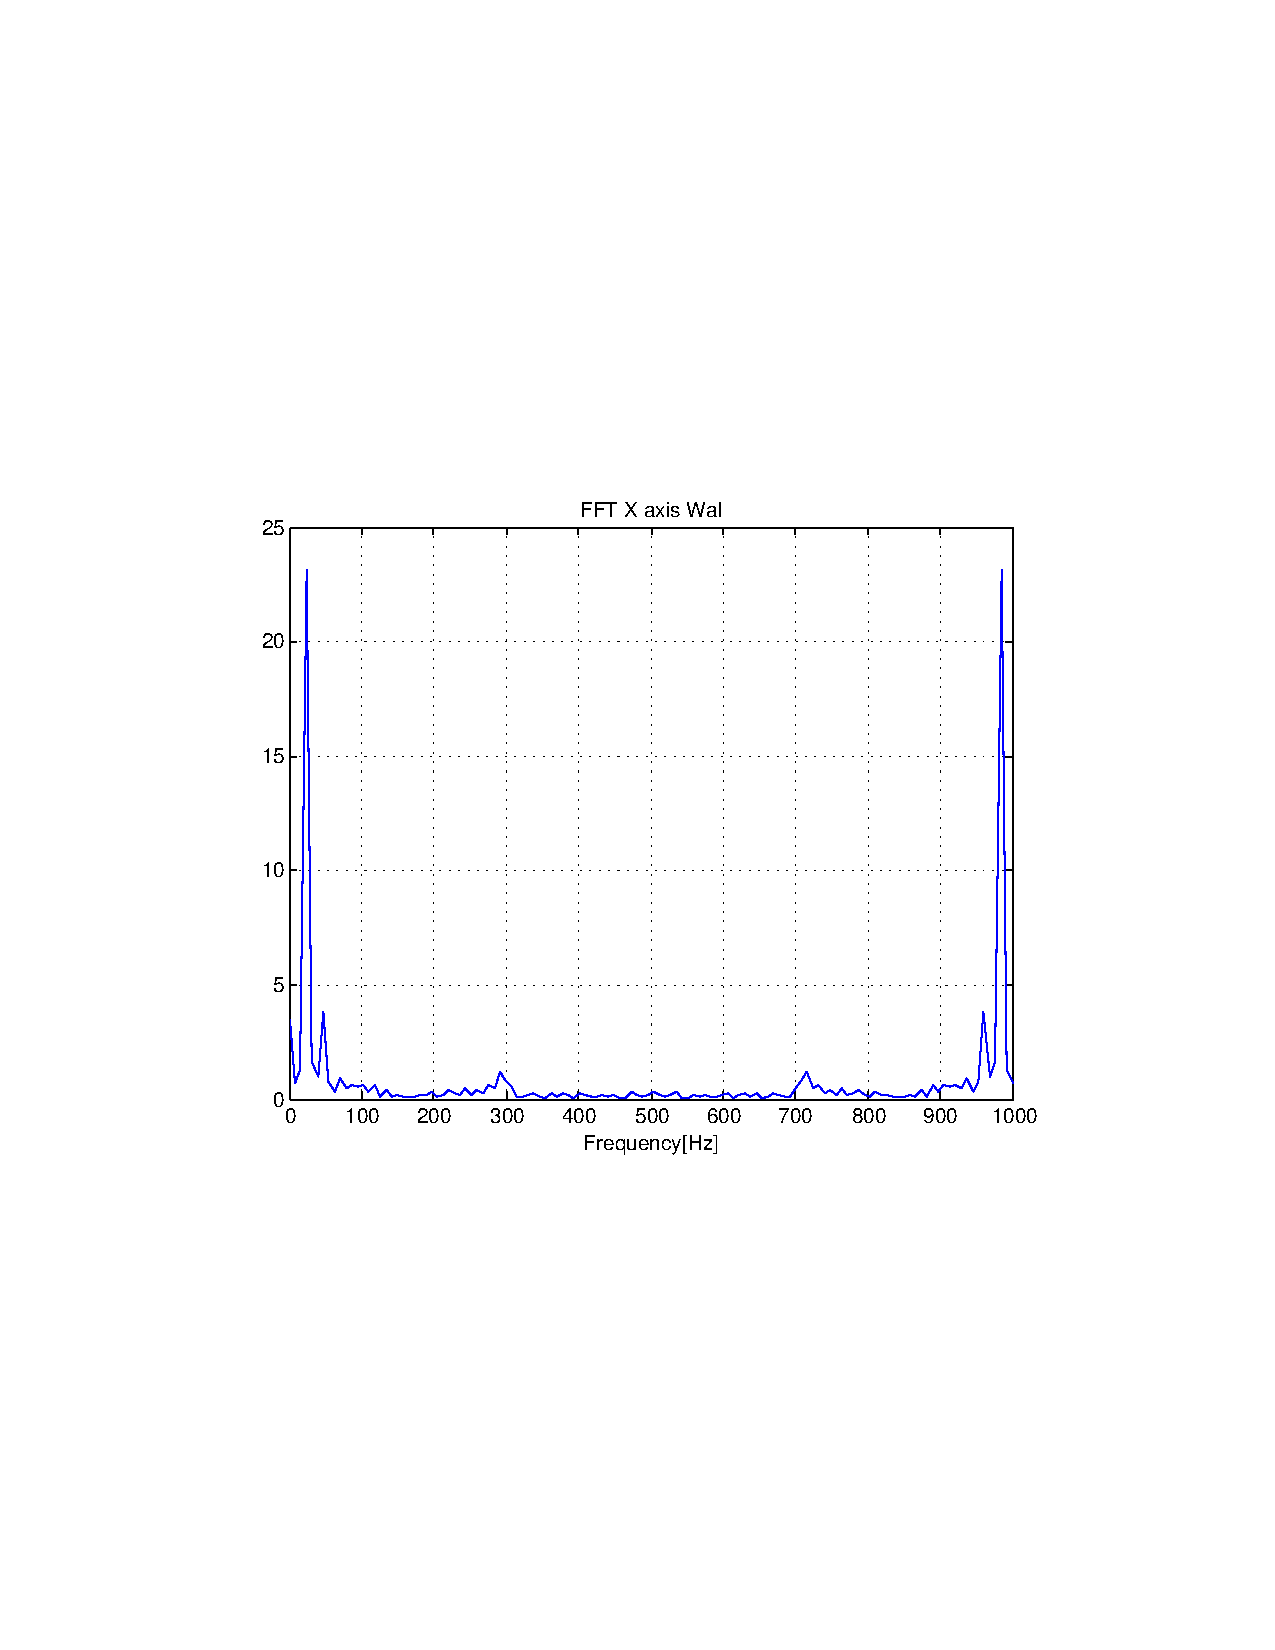
\includegraphics[trim=5cm 8.5cm 5cm
                8.5cm,width=10cm]{../res/img/a_fft_wal_x.pdf}
            \end{center}
            \caption{FFT przyśpieszeń na wale w osi X}
            \label{rys:fwalx}
        \end{figure}
        \begin{figure}[!htb]
            \begin{center} 
                \includegraphics[trim=5cm 8.5cm 5cm
                8.5cm,width=10cm]{../res/img/a_fft_ob_x.pdf}
            \end{center}
            \caption{FFT przyśpieszeń na obudowie w osi X}
            \label{rys:fobx}
        \end{figure}
        
        \newpage
        
        \begin{figure}[!htb]
            \begin{center} 
                \includegraphics[trim=5cm 8.5cm 5cm
                8.5cm,width=10cm]{../res/img/a_fft_wal_y.pdf}
            \end{center}
            \caption{FFT przyśpieszeń na wale w osi Y}
            \label{rys:fwaly}
        \end{figure}
        \begin{figure}[!htb]
            \begin{center} 
                \includegraphics[trim=5cm 8.5cm 5cm
                8.5cm,width=10cm]{../res/img/a_fft_ob_y.pdf}
            \end{center}
            \caption{FFT przyśpieszeń na obudowie w osi Y}
            \label{rys:foby}
        \end{figure}
        
        \newpage
        
        \begin{figure}[!htb]
            \begin{center} 
                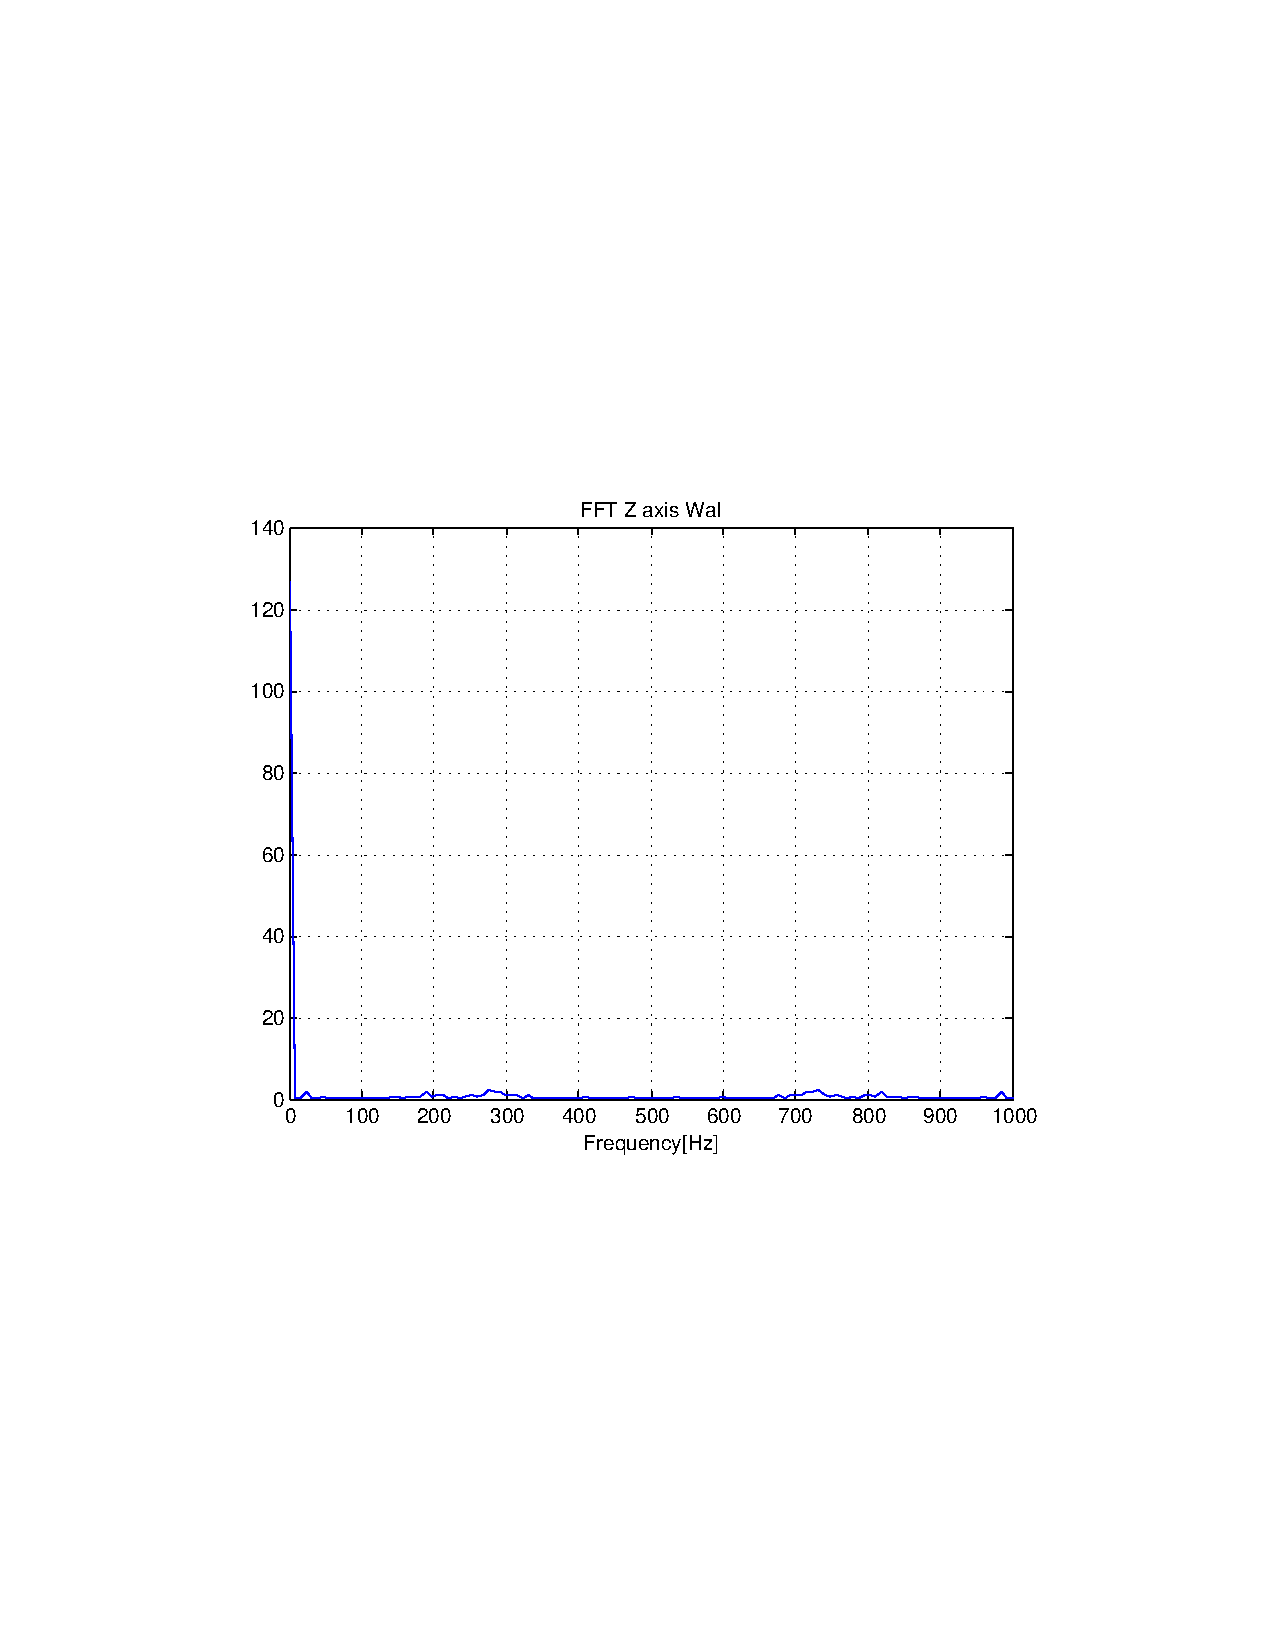
\includegraphics[trim=5cm 8.5cm 5cm
                8.5cm,width=10cm]{../res/img/a_fft_wal_z.pdf}
            \end{center}
            \caption{FFT przyśpieszeń na wale w osi Z}
            \label{rys:fwalz}
        \end{figure}
        \begin{figure}[!htb]
            \begin{center} 
                \includegraphics[trim=5cm 8.5cm 5cm
                8.5cm,width=10cm]{../res/img/a_fft_ob_z.pdf}
            \end{center}
            \caption{FFT przyśpieszeń na obudowie w osi Z}
            \label{rys:fobz}
        \end{figure}
        
        \newpage
        
        Korzystając z widma sygnału przyspieszenia w osi X , można oszacować
        prędkość obrotową silnika generującego mierzone drgania. Jako że
        dominującym prążkiem jest częstotliwość $31.5[Hz]$, stąd można
        przypuszczać, iż silnik obracał się z prędkością ok.
        $1890[\frac{obr}{min}]$.
    \end{subsection}	
\end{section}

\begin{section}{Wnioski}
    Na podstawie częstotliwości drgań generowanych przez wirujące elementy
    maszyn, jesteśmy w stanie wyznaczyć ich przybliżoną prądkość obrotową. Na podstawie
    odczytów z czujnika przyspieszenia, w krótkich odcinkach czasu, jesteśmy
    również w stanie określić względną zmianę prędkości, a nawet
    przemieszczenia.
\end{section} 

\begin{section}{Wykaz aparatury}   
	\begin{enumerate}
	  \item Komputer z systemem operacyjnym Windows XP lub wyższym
	  \item Karta pomiarowa NI6221 wraz z płytką łączeniową
	  \item Oprogramowanie DASY Lab wraz ze sterownikami do karty (NI - DAQmx)
	  \item Wzmacniacz pomiarowy MVD 2555
	  \item Akcelerometr tensometryczny typu BWH
	  \item Zintegrowany pojemnościowy akcelerometr 3-osiowy na bazie ADXL320EB
	  \item Zasilacz stabilizowany +5V do akcelerometru ADXL320EB
	\end{enumerate}
\end{section}

\end{document}